\documentclass{article}
\usepackage[a4paper, left=1.5cm, right=1.5cm, top=1cm, bottom=2cm]{geometry}
\usepackage{tikz,tcolorbox}
\usepackage{amsmath}
\usepackage[table,xcdraw]{xcolor}
\usepackage{listings}
\usepackage{array,multirow} % For customizing tables
\usepackage{booktabs} % For better horizontal lines
\usepackage{makecell}
\setlength{\parindent}{0pt}

\usepackage{amssymb}
\tcbuselibrary{skins, breakable, theorems}

\definecolor{myblue}{HTML}{10C2C4}

\newtcolorbox{prettyBox}[2]{
  enhanced,
  colback=white!90!#2,   % Background color based on the second parameter (color)
  colframe=#2!60!black,  % Frame color based on the second parameter (color)
  coltitle=white,        % Title color (white)
  fonttitle=\bfseries\Large,
  title=#1,              % Title from the first parameter
  boxrule=1mm,
  arc=0.5mm,
  drop shadow=#2!35!gray, % Drop shadow color based on the second parameter (color)
}

\usepackage{listings}
% Define the style for C code
\lstdefinestyle{cstyle}{
    language=C,
    basicstyle=\ttfamily\small,
    keywordstyle=\color{blue}\bfseries,
    stringstyle=\color{red},
    commentstyle=\color{green!50!black}\itshape,
    numbers=left,
    numberstyle=\tiny\color{gray},
    stepnumber=1,
    breaklines=true,
    frame=tb,
    tabsize=4,
    showstringspaces=false,
    captionpos=b
}

\lstdefinestyle{cmd}{
 basicstyle=\ttfamily,
 backgroundcolor=\color{lightgray!20},
 frame=single
}

\lstdefinestyle{javaStyle}{
    language=Java,
    basicstyle=\ttfamily\footnotesize,   % Font style and size
    numbers=left,                       % Line numbers on the left
    numberstyle=\tiny\color{gray},       % Style for line numbers
    stepnumber=1,                        % Line number step
    numbersep=5pt,                       % Distance of numbers from the code
    backgroundcolor=\color{white},       % Background color of the listing
    showspaces=false,                    % Don't show spaces
    showstringspaces=false,              % Don't show spaces in strings
    showtabs=false,                      % Don't show tab characters
    frame=single,                        % Add a frame around the code
    rulecolor=\color{black},             % Color of the frame
    tabsize=2,                           % Tab size
    captionpos=b,                        % Position of the caption (bottom)
    breaklines=true,                     % Automatically break long lines
    breakatwhitespace=true,              % Break at white space
    escapeinside={\%*}{*)},              % Allows comments in LaTeX inside the listing
    keywordstyle=\color{blue},           % Keyword color
    commentstyle=\color{green},          % Comment color
    stringstyle=\color{red},             % String color
}



\lstdefinestyle{pythonstyle2}{
    language=python,                    % Language set to Python
    basicstyle=\ttfamily\footnotesize,   % Change basic font size
    keywordstyle=\color{blue}\bfseries, % Different keyword style
    stringstyle=\color{red},         % Different string color
    commentstyle=\color{green!60!black}\itshape, % Adjust comment color
    numbers=left,                       % Line numbers on the left
    numberstyle=\tiny\color{gray},      % Smaller number font and color
    stepnumber=1,                       % Number each line
    frame=single,                       % Single frame around code
    tabsize=4,                          % Adjust tab size
    showstringspaces=false,             % Do not show spaces in strings
    captionpos=b,% Position of caption
    breaklines=true,
    inputencoding=utf8
}




\begin{document}
\begin{center}
    \Huge{\textbf{\underline{Chapter 1: Introduction}}}
\end{center}

\vspace{0.35cm}


\section{Numerical Algorithm (Numerical Method)}
\begin{prettyBox}{Numerical Algorithm}{mygreen}
A Numerical Algorithm provides an approximate solution and is used to solve problems involving large amounts of data. The algorithm is based on a well-defined iterative sequence, starting with an initial solution that progressively converges toward the desired result with each iteration.

\[
\begin{cases}
    \hspace{0.1cm}(U_n) & \hspace{-0.1cm}n \geq 0 \\[0.15cm]
    \hspace{0.1cm}S_0 & \hspace{-0.3cm} \text{Initial Solution (Starting Point)}
\end{cases}
\]
\end{prettyBox}
\vspace{0.35cm}

\section{Convergence Speed (Order of Convergence)}
\begin{prettyBox}{Convergence Speed}{mygreen}
The number of iterations required to find the solution we are looking for:
\begin{itemize}
    \item Linear Order: 1 (slow)
    \item Quadratic Order: 2 (faster)
    \item \(>>\) 2 (very fast)
\end{itemize}
\end{prettyBox}

\vspace{0.35cm}

\section{Interpolation}
\begin{prettyBox}{Interpolation}{mygreen}
Estimates the value between two known points of a function allowing for a smoother representation of the function's behavior.
\end{prettyBox}

\vspace{0.35cm}

\section{Approximation}
\begin{prettyBox}{Approximation}{mygreen}
Approximates the formula of a function from a set of values, with the objective of finding a simpler function that represents the general trend of the data, even if it doesn't pass through every point exactly.
\end{prettyBox}

\vspace{0.35cm}

\section{Error}
\begin{prettyBox}{Error}{mygreen}
An error represents the difference between the actual solution and the computed result. It indicates how far we are from the true solution. There are two cases:
\begin{itemize}
    \item \textbf{Evaluation}: We know the exact solution, so we can directly calculate the error:
        \[   \boxed{E_r = |\overline{x} - x_{\text{app}}|} \]
    \item \textbf{Estimation}: We don't know the exact solution, so we only have an estimate of the error, based on the output of the algorithm:
        \[      \boxed{E_r = |\overline{x} - x_{\text{app}}| \leq \text{Algo}} \]
\end{itemize}

Where:
\begin{itemize}
    \item \(E_r\) : The error value.
    \item \(\overline{x}\) : The exact solution.
    \item \(x_{\text{app}}\) : The approximate solution.
    \item Algo : The error value found by the algorithm.
\end{itemize}
\end{prettyBox}

\vspace{0.35cm}

\section{Optimization}
\begin{prettyBox}{Optimization}{mygreen}
Optimization in numerical algorithms refers to two things:
\begin{itemize}
    \item \textbf{Error}: We aim to minimize the error in order to achieve the most accurate approximate solution.
    \item \textbf{Convergence Speed}: The higher the order of convergence, the less time the algorithm will take to converge to the solution we are looking for.
\end{itemize}
\end{prettyBox}

 
\newpage
\begin{center}
    \Huge{\textbf{\underline{Chapter 2: Design Pattern}}}
\end{center}

\setcounter{section}{0}

\vspace{0.35cm}


 
\newpage
\begin{center}
    \Huge{\textbf{\underline{Chapter 3: MVC \& PAC}}}
\end{center}

\setcounter{section}{0}

\vspace{0.3cm}


\section{Architectural Design Pattern}
\begin{prettyBox}{Architectural}{myblue}
So far, we’ve only seen the Gang of Four design patterns, which help to implement parts of a project.  
Architectural design patterns such as MVC and PAC structure the entire project by applying the patterns we’ve previously learned.
\end{prettyBox}

\vspace{0.2cm}

\section{Some Terminologies}
\begin{prettyBox}{Definitions}{myblue}
Before explaining MVC and PAC, it is important to understand the following terms:
\begin{itemize}
    \item \textbf{Model (Abstraction)}: the application’s internal data and processing logic.
    \item \textbf{View (Presentation)}: what the user sees and interacts with (Interface).
    \item \textbf{Controller}: the event handler that mediates between the Model and the View.
\end{itemize}
\end{prettyBox}

\vspace{0.2cm}
\section{MVC \& Pac}

\subsection{MVC}
\begin{prettyBox}{MVC (Model View Controller)}{myblue}
The MVC divides the project into 3 categories: Model, View and Controller, but it also imposes how 
these parts interact with each other. It has a circular communication:
\begin{enumerate}
    \item User interacts with the View (interface).
    \item The View sends the user’s request to the appropriate Controller.
    \item Controller changes the Model accordingly.
    \item Model notifies the View.
    \item View updates.
\end{enumerate}
\end{prettyBox}

\vspace{0.1cm}
\begin{center}
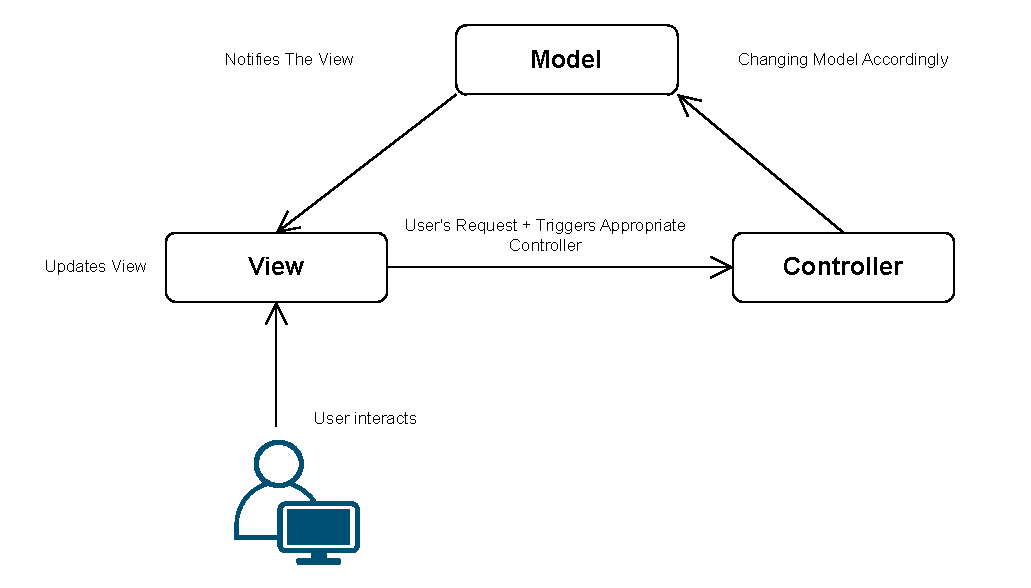
\includegraphics[height=0.25\textheight]{Chapters/MVC_PAC/mvc1.drawio.pdf}
\end{center}

\subsection{PAC}
\begin{prettyBox}{PAC (Presentation Abstraction Controller)}{myblue}
The PAC divides the project into 3 categories: Abstraction (Model), Presentation (View) and Controller, but it also imposes how 
these parts interact with each other. It has a linear communication:
\begin{enumerate}
    \item User interacts with the View (interface).
    \item The View sends the user’s request to the appropriate Controller.
    \item Controller changes the Model accordingly.
    \item Model notifies the Controller.
    \item Controller notifies the View.
    \item View updates.
\end{enumerate}   
\end{prettyBox}

\vspace{0.1cm}
\begin{center}
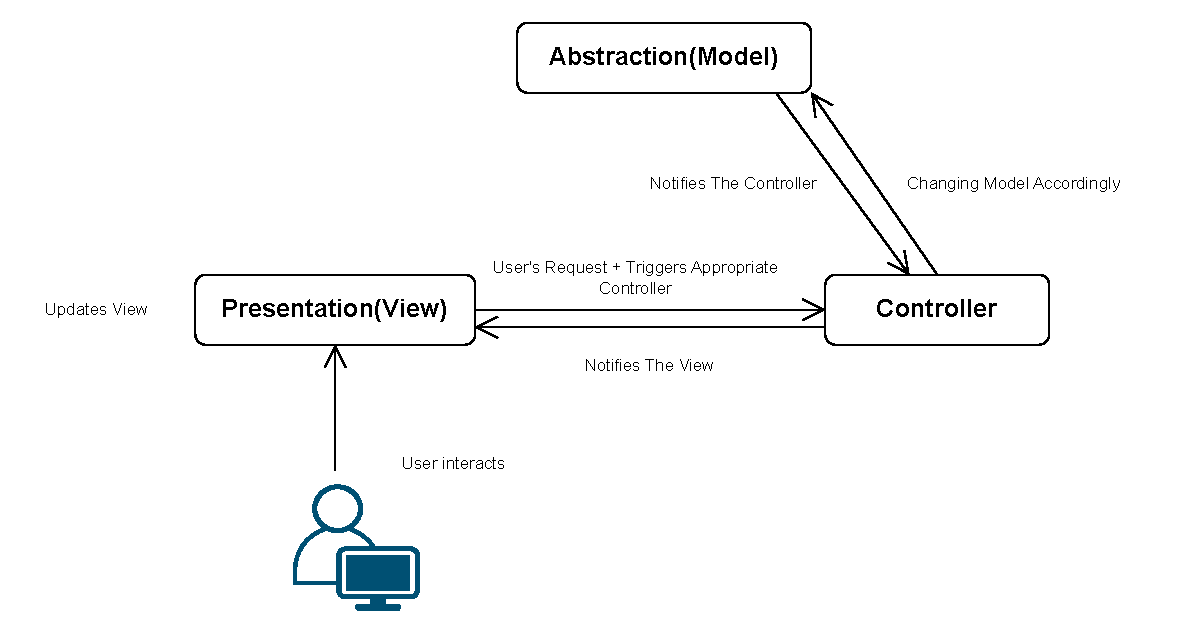
\includegraphics[height=0.25\textheight]{Chapters/MVC_PAC/pac1.drawio.pdf}
\end{center}

\vspace{0.25cm}

\begin{prettyBox}{Note}{red}
Just dividing a project into Model, View and Controller isn't enough to say that it follows MVC or PAC. The way these parts communicate is important too.
\end{prettyBox}

\vspace{0.5cm}

\subsection{Difference Between MVC \& PAC}
\begin{prettyBox}{Difference}{red}
Even though both divide the project into three parts, they differ in how these parts communicate. At first they work
the same: the user interacts with the View, which sends the request to the Controller, which changes the Model. Then they
differ. In MVC, the Model notifies the View directly, creating a circular flow. In PAC, the Model notifies the
Controller, which then notifies the View, creating a linear flow.
\end{prettyBox}

\newpage
\subsection{UML}
\subsubsection{MVC}

\vspace{0.25cm}
\begin{center}
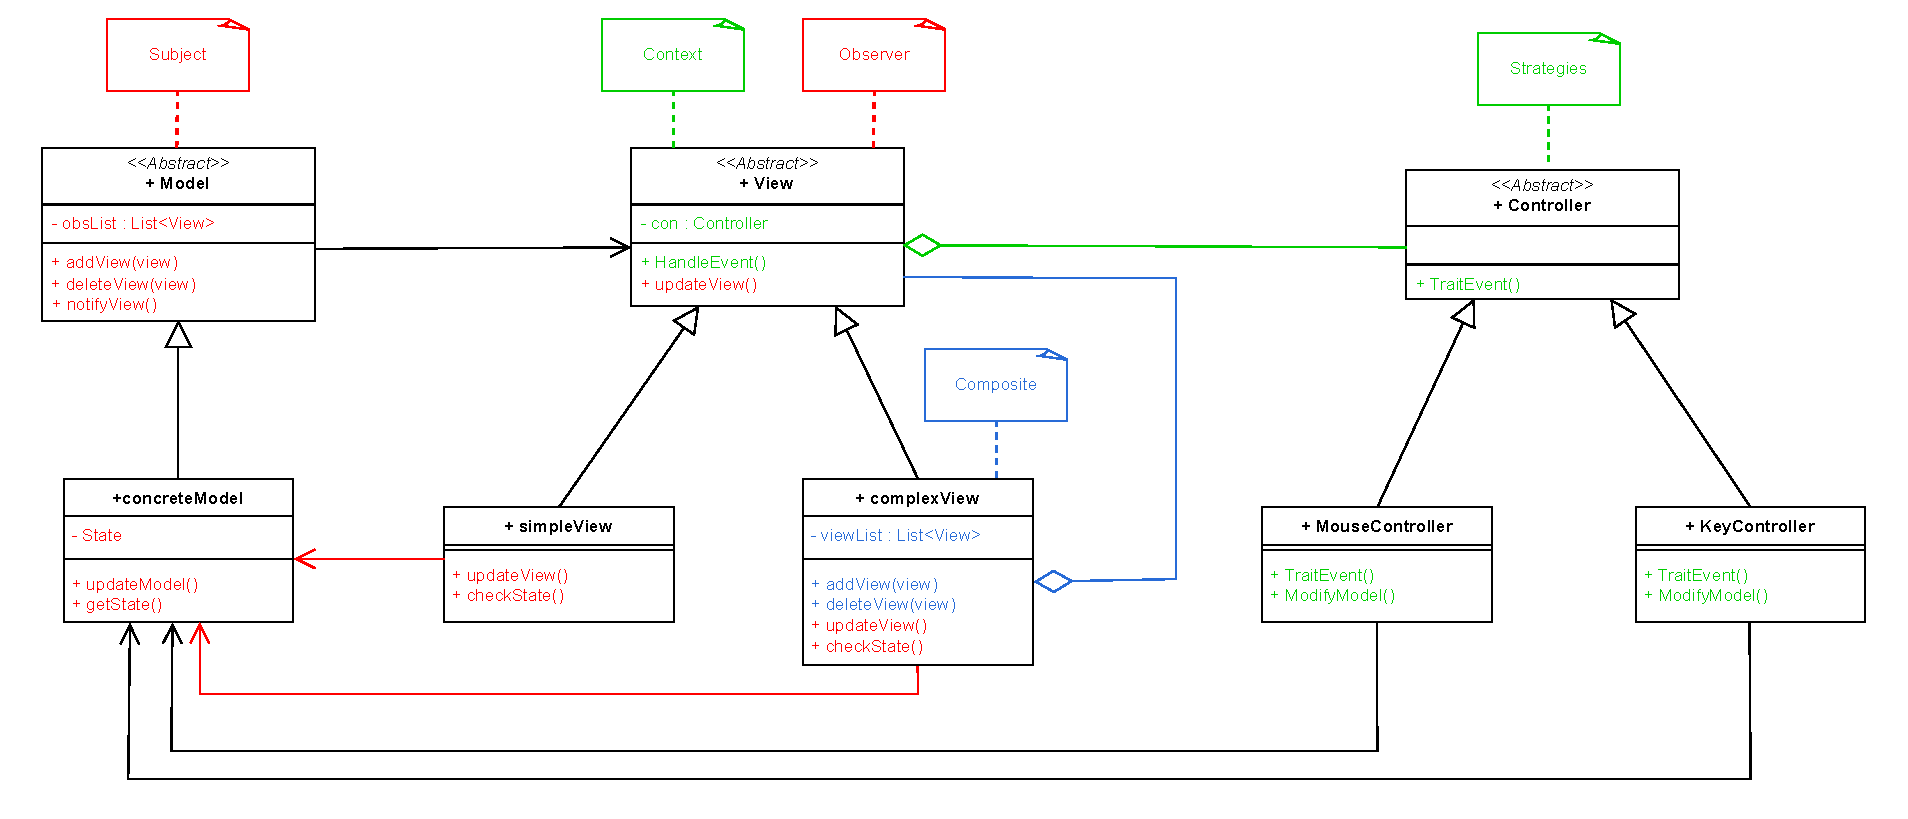
\includegraphics[height=0.25\textheight]{Chapters/MVC_PAC/mvc2.drawio.pdf}
\end{center}

\vspace{0.25cm}


\begin{prettyBox}{Explication}{myblue}
The View uses the Composite design pattern to organize views into a hierarchy of simple and nested views.\\[0.15cm]
The user sees and interacts only with the View, triggering events at runtime, so we apply the Strategy design
pattern between the View and Controller: the View is the context, holds a reference to the Controller, and defines
a \texttt{handleEvent()} method that calls the Controller’s \texttt{traitEvent()}, while each Controller implements
a strategy to update the Model based on the user event. Inside \texttt{traitEvent()} \texttt{modifyModel()} is called and invokes
the Model’s \texttt{updateModel()} method.\\[0.15cm]
We use the Observer design pattern between the Model and View because the Model holds data that external classes
(views) are interested in and that can change at runtime. When \texttt{updateModel()} is called, it runs \texttt{notifyView()},
which loops through all observers(views) of \texttt{obsList} and calls each observer’s \texttt{updateView()} which uses \texttt{checkState()} to call \texttt{getState()}.
\end{prettyBox}

\newpage
\subsubsection{PAC}

\vspace{0.25cm}
\begin{center}
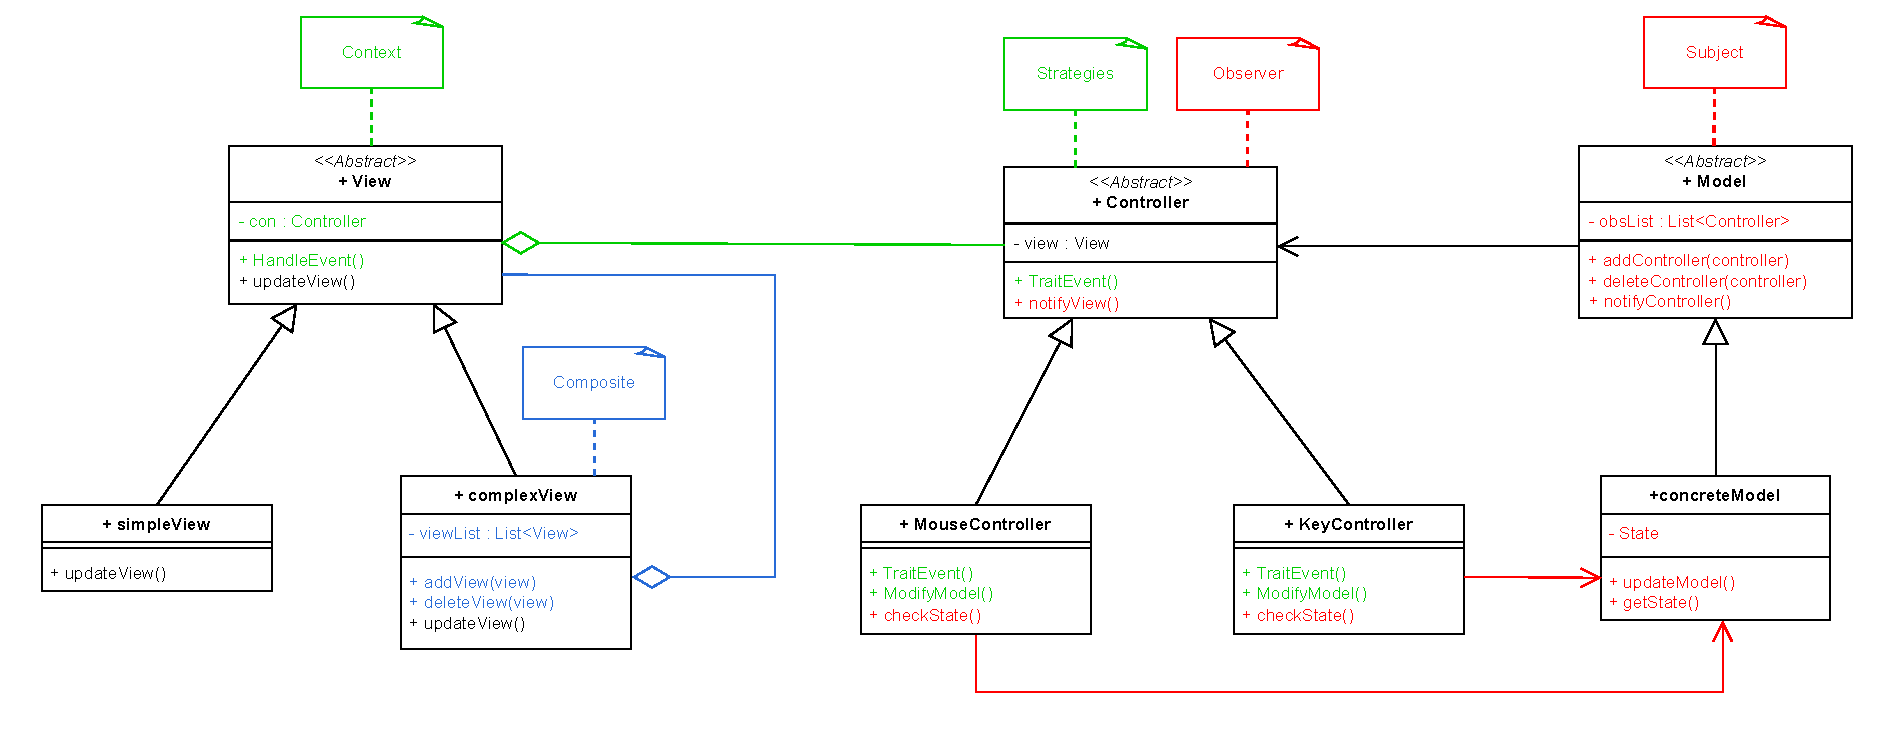
\includegraphics[height=0.25\textheight]{Chapters/MVC_PAC/pac2.drawio.pdf}
\end{center}

\vspace{0.25cm}
\begin{prettyBox}{Explication}{myblue}
The View uses the Composite design pattern to organize views into a hierarchy of simple and nested views.\\[0.15cm]
The user sees and interacts only with the View, triggering events at runtime, so we apply the Strategy design
pattern between the View and Controller: the View is the context, holds a reference to the Controller, and defines
a \texttt{handleEvent()} method that calls the Controller’s \texttt{traitEvent()}, while each Controller implements
a strategy to update the Model based on the user event. Inside \texttt{traitEvent()} \texttt{modifyModel()} is called and invokes
the Model’s \texttt{updateModel()} method.\\[0.15cm]
We use the Observer design pattern between the Model and controller because the Model holds data that external classes
(controller) are interested in and that can change at runtime. When \texttt{updateModel()} is called, it runs \texttt{notifycontroller()} 
which loops through all observers(controllers) of \texttt{obsList} and calls each observer’s \texttt{notifyView()} which calls 
the \texttt{checkState()} method , and the \texttt{updateView()} of the view object held in controller class.
\end{prettyBox}


 
\end{document}
